%%%%%%%%%%%%%%%%%%%%%%%%%%%%%%%%%%%%%%%%%%%%%%%
%%%%%%%%%%%%%%%%%%%%%%%%%%%%%%%%%%%%%%%%%%%%%%%
%%%%%%%%%%%%%%%%%%%%%%%%%%%%%%%%%%%%%%%%%%%%%%%
\setcounter{section}{2}\section{日本が狙うサイエンス}\label{c08.s3}

SKAと同じ帯域の観測は日本では限られるため、SKAが狙う具体的観測に直接つながるような日本の独自研究はまだ少ない。そのため、本節の日本が狙うSKAサイエンスにおいては、科学検討班メンバーのこれまでの研究を基礎としたときに、それを独自性としてSKAでどのような研究が可能か検討した。


%%%%%%%%%%%%%%%%%%%%%%%%%%%%%%%%%%%%%%%%%%%%%%%
%%%%%%%%%%%%%%%%%%%%%%%%%%%%%%%%%%%%%%%%%%%%%%%
\subsection{星間媒質における中性水素原子雲の役割と観測の重要性}
\label{c08.s4.ss1}

\paragraph{中性水素原子雲の役割}

H\,\textsc{i}雲は分子雲の原材料であると考えられているが、分子雲はその名称が示すように主にCO分子輝線で観測されており、原材料であるH\,\textsc{i}雲が分子雲の、特に星形成活動にどのような影響を与えているのかについては全く理解されていない。近年の分子雲形成シミュレーションは原材料であるH\,\textsc{i}雲の降着が分子雲の超音速乱流の主要駆動要因になっていることを示唆しており、さらに、これまで観測されてこなかった乱流エネルギーの中性水素原子が担う成分は分子のそれを桁で凌駕するほど強く、分子雲での星形成を本質的にコントロールしていることを示唆している\citep{2012ApJ...759...35I}。

\paragraph{中性水素原子雲の観測の重要性}

このような新しい星形成描像を確認する為には分子雲を単に分子輝線で観測するだけでは不十分であり、中性水素原子まで含めたでシステム全体を観測することが必要不可欠である。さらに、近年の若い超新星残骸の磁気流体シミュレーションは、分子雲やH\,\textsc{i}雲と超新星衝撃波の相互作用が、乱流励起を介して宇宙線加速を促進することを示しており、また宇宙線と雲の相互作用で発生するガンマ線放射を通して宇宙線のプローブとしての役割を期待することができる。SKAによって若い超新星残骸周辺の中性水素原子観測が進展すれば、X線やガンマ線放射と比較することによって通常の方法では困難な宇宙線陽子の加速効率を測定する道を開くことができる\citep{2012ApJ...744...71I}。

%%%%%%%%%%%%%%%%%%%%%%%%%%%%%%%%%%%%%%%%%%%%%%%
%%%%%%%%%%%%%%%%%%%%%%%%%%%%%%%%%%%%%%%%%%%%%%%
\subsection{ALMAや野辺山45mなどのミリ波・サブミリ波との相補性}
\label{c08.s4.ss2}

\paragraph{ミリ波・サブミリ波による星間物質研究}

日本ではミリ波・サブミリ波による星間物質の研究が盛んである。特に様々な分子輝線サーベイや、ミリ波・サブミリ波領域でのmulti transition観測による研究は、星間物質の異なる物理状態(密度や温度、紫外線強度や進化の段階など)を調べることに確実に力を発揮する。

\paragraph{ミリ波・サブミリ波による星間物質研究の例}

一例として、誕生したばかりの原始星は濃い分子雲コアに埋もれており、近赤外線より短い波長では見通すことができない。しかし質量降着現象を伴う中心星からの放射は、センチ波連続波を使えば検出可能で、さらに強いメーザー現象を起こすこともある。また激しい分子流やジェットを伴うことで濃い分子ガスエンベロープを一部破壊、衝撃波領域が観測される。また中心星の近傍にはホットコアと呼ばれる高密度で温かい分子ガス塊が存在し、様々な分子が形成されたり、星の周囲をケプラー回転する円盤も形成される。

\paragraph{SKAへの期待}

このように数100 AUから0.1 pc程度にわたる空間スケール中に、異なる形態の変化に富んだ物質が存在しており、これらを総合的に観測理解するためには、ミリ波・サブミリ波の望遠鏡とのシナジーが必要不可欠である。SKAにより、H\,\textsc{i}ガス、OH分子や、電離領域からの再結合線や電波連続波の情報が与えられることで、広いダイナミックレンジで星間ガスの物理状態を特定することが可能となる。


%%%%%%%%%%%%%%%%%%%%%%%%%%%%%%%%%%%%%%%%%%%%%%%
%%%%%%%%%%%%%%%%%%%%%%%%%%%%%%%%%%%%%%%%%%%%%%%
\subsection{臼田64m鏡H\,\textsc{i}観測}
\label{c08.s4.ss3}

\paragraph{国内H\,\textsc{i}観測のニーズ}

H\,\textsc{i}輝線は電波天文学において重要な輝線であるが、これまで日本国内ではH\,\textsc{i}輝線を観測する科学運用に可能な望遠鏡が存在せず、基本的に海外の装置を使うしかなかった。もし国内に科学運用可能なH\,\textsc{i} 21cm線観測のできる装置があれば、国内研究者にとってH\,\textsc{i}観測がさらに身近になり、H\,\textsc{i}をターゲットにした研究者層を厚くすることに繋がるだろう。例えばこれまで大口径望遠鏡を用いた全天H\,\textsc{i}サーベイが進められてきたが、速度分解能は1 km/sである。しかし星間ガスの研究には0.1 km/sオーダーの速度分解能が必要であり、高速度分解能によるH\,\textsc{i}観測のニーズはある。前節までに紹介したSKAでのH\,\textsc{i}輝線観測の将来性から、国内のH\,\textsc{i}観測のニーズはさらに高まると予想される。

\paragraph{臼田H\,\textsc{i}パイロット観測}

臼田宇宙空間観測所64m鏡は日本最大口径の望遠鏡であり、LバンドからKバンドの受信機が搭載されている。世界的に見ても十分対抗できる大型単一鏡である。オーストラリアParkes 64m望遠鏡と同じ口径の望遠鏡であり、Parkesは南天、臼田が北天を走査するという相補性が期待できる。さらに北天は銀河円盤の外側領域を含んでいるという特徴がある。臼田64m鏡はこれまで衛星管制を主に担ってきたため、科学運用にはほとんど使われてこなかった。しかし2013年頃から有志によって科学運用についての検討を開始し、2014年1月にワークショップを開き、科学運用に関する議論を行った。これを機にH\,\textsc{i}輝線観測を実現するためのワーキンググループが結成され、H\,\textsc{i}輝線観測のための システム整備を始め、試験観測を行ってきた。2014 年度には一般にH\,\textsc{i} 21cm線観測で行われる周波数スイッチを実装することに成功した。周波数スイッチによる周波数特性補正、地球回転によるドップラー効果を補正する解析システムを開発した。引き続き性能評価を進め、ユーザーフレンドリーなシステムとなるよう整備を進めている。現在の問題点としては、システム雑音温度が400Kと非常に高いため、これを改善することが課題である。また連続波観測、偏波観測を可能にするシステムを開発したいと考えている。


%%%%%%%%%%%%%%%%%%%%%%%%%%%%%%%%%%%%%%%%%%%%%%%
%%%%%%%%%%%%%%%%%%%%%%%%%%%%%%%%%%%%%%%%%%%%%%%
\subsection{パルサーグループからもたらされる精密情報の活用}
\label{c08.s4.ss4}

\paragraph{はじめに}

詳細な説明は第\ref{pulsar}章と第\ref{astrometry}章に譲るが、パルサーは天の川銀河とその周辺の星間物質、特に電離ガスと付随する磁場の分布を精密に把握するためのプローブとして期待されている。

\paragraph{パルサータイミング}

パルサーの観測では、非常に精度の高いパルサーからのパルス信号の周期とその時間変化率を精密に測定する(パルサータイミング)。SKAでは、約2週間間隔で約48時間掛けて約2000個のミリ秒パルサーを観測し、パルス周期を10~nsの精度で測定することを想定している。これによりパルス周期の年周変化(とアストロメトリに基づく年周視差法)からパルサーまでの距離を精度良く推定できる。

\paragraph{パルサー観測から得られる星間物質の観測量}

またパルサーのパルスは、広い周波数範囲にわたって分光される。そのデータから、低い周波数ほどパルス到達時間が遅くなる比率を示す Dispersion Measure (DM)、周波数に伴って直線偏波角が回転していく比率を示す Rotation Measure (RM)を測定することができる。それらはそれぞれ、星間電子密度、星間電子密度と磁場の積、をパルサー方向に積分したものに相当する。従って、パルサーまでの距離が既知であれば、パルサー方向の星間電子密度、星間電子密度と磁場の平均値を推定できる。NE2001と呼ばれる天の川銀河中の電子密度モデルは\citep{2002astro.ph..7156C}、距離が既知のパルサーに対してDMデータと組み合わせて構築されたものである。SKAでは、ほぼ同じ視線方向で複数のパルサーに対するタイミング観測が実施される。そのような状況では、これらパルサー間においてRMとDMそれぞれの差の比からパルサー間の平均磁場、ひいては同じ領域の電子密度を推定できる。さらに、低い周波数ほどパルスの時間幅が伸びる比率を示す Scattering Measure (SM)も測定されれば、星間プラズマの乱流スペクトルの推定もできる。また、パルサー固有運動が引き起こすDMの時間変化によっても、乱流の様子を把握することができる。手前の星間ガスによる21~cm線や再結合線、分子線スペクトルの吸収線も想定される。

\paragraph{パルサーの分布}

パルサーはもともと比較的軽い大質量星の超新星爆発によって形成されたものであり、その寿命も$10^{7}$年未満とされている。しかし、超新星爆発の非対称性によって高速で蹴り出され(pulsar kick)、1000~km~s$^{-1}$もの速さで移動するパルサーも見つかっている。従って、天の川銀河の中でのパルサーの分布は、その発祥となる星形成領域から遠く離れ、星形成領域の分布よりもやや厚みを持っていると考えられる。このように、H\,\textsc{i}同様、広く天の川の星間ガスの分布を把握するのにパルサーは有用である。

\paragraph{SKA観測に向けた技術的課題}

ただし、精密な分光による吸収線の観測は、リアルタイムでのデータ処理能力に掛かっている。パルサーの観測ではタイミング観測が主流となるので保存される観測データの積分時間間隔が極端に短く(マイクロ秒程度)、これと同時に多数の分光チャンネル(25万分光点、SKA1-MIDで視線速度分解能1~km~s$^{-1}$程度)を得ることは難しい。同じパルサー観測データを別途、積分時間を長くする代わりに高い周波数分解能で処理するパスも、構築することが必要であろう。


%%%%%%%%%%%%%%%%%%%%%%%%%%%%%%%%%%%%%%%%%%%%%%%
%%%%%%%%%%%%%%%%%%%%%%%%%%%%%%%%%%%%%%%%%%%%%%%
\subsection{銀河進化グループがもたらす星形成の知見}
\label{c08.s4.ss5}

\paragraph{星間物質と銀河進化}

日本の優位性のひとつとして、星間物質研究との境界領域の研究も幅広く行われている点がある。星間物質の研究は、銀河進化の研究の礎となることはいうまでもない。銀河進化については日本SKA銀河進化科学検討班が議論を重ねてきている。銀河進化研究の黎明期から現在にわたるまで一貫してその中心的話題となっている課題は星形成史、すなわち銀河の星間物質においてガスが星に転化する過程の時間進化である。銀河研究における限界はその距離によって決まっている。素過程としての銀河進化の物理学は星間物質の研究と原理的に同一であるはずだが、系外銀河は遠方に存在するため角分解能の限界により、星間物理のレベルでの観測はこれまで事実上不可能であった。このような事情から、銀河の研究はまず全光度、星質量、ガス質量、力学質量等のグローバルな物理量の間に存在する経験則を発見し、それをある程度単純な物理法則で説明するというアプローチが取られることが多かった。しかし、この方法論にはおのずと限界があり、今日でも銀河の星形成研究は星間物理学で常識となっている知識との有機的な結合は全くできていないと言っても過言ではない。

\paragraph{SKAへの期待}

SKAはこの観測的な限界を突破し、劇的な進展をもたらす。SKAの角分解能は現時点での星間物理に匹敵するまでは及ばないとしても、それに近い空間分解をすることができ、銀河の内部的環境の違いと星形成に関する物理の依存性を議論することができるようになる。これがもたらすブレイクスルーは、銀河進化研究と星間物質研究の間のミッシングリンクをつなぐ真の意味での有機的研究を生むと期待できる。

\paragraph{日本のサイエンスの狙い}

具体的なテーマとして最も重要なのは、星の原料である中性水素原子ガスから分子ガス、分子雲を経て恒星に至る過程を物理環境の関数として表現することである。銀河進化サブグループではこの点に特に注目しており(\S \ref{galaxy}参照)、ガスの原子分子相転移を空間的、時間的にトレースすることを中心的課題として追及する。これは明らかに星間物質研究の中心的課題でもあり、現時点で明らかになっている星間物理の局所的性質が、何桁も大きい銀河の大局的星形成に見られる経験則をどう形作っていくかを明らかにする研究となる。標語的にいえば、銀河の星形成研究はSKAによって初めて物理学として成熟することになるといえるだろう。


%%%%%%%%%%%%%%%%%%%%%%%%%%%%%%%%%%%%%%%%%%%%%%%
%%%%%%%%%%%%%%%%%%%%%%%%%%%%%%%%%%%%%%%%%%%%%%%
\subsection{宇宙磁場グループが明かす電離ガスの情報}
\label{c08.s4.ss6}

\paragraph{SKA時代の偏波観測}

国際SKA宇宙磁場科学検討班では、背景偏波源のRMサーベイを最優先課題としている。現在の最大の偏波源カタログでは1平方度あたり平均1つの偏波源が観測されているが、これが数百から数万へと激増する見込みであり(図\ref{c06.s2.ss1.f1})、密なRMグリッドを天球に得ることができるようになる。加えて日本SKA宇宙磁場科学検討班では、偏波解消とファラデートモグラフィーに注目している(\S \ref{magnetism}参照)。これらは広帯域な偏波観測データから視線上の物質構造の情報を直接抽出できる潜在能力がある。

\paragraph{偏波観測サイエンス}

偏波の起源が何であれ、星間空間を通過してきた偏波は星間物質の情報を含んでいる。RMグリッドは天球面方向の、偏波解消とトモグラフィーは視線方向の情報をもたらす。ゆえにRMグリッド、偏波解消、そしてトモグラフィーを組み合わせれば、視線上の別の成分の寄与を区別しながら、星間物質(直接的にはWIMの熱的電子と磁場、ならびに宇宙線電子)の3次元構造をこれまでにない精度で明らかにできるだろう。そのデータを用いて果たせるサイエンスとして、日本SKA宇宙磁場科学検討班は星間・銀河磁場とそれに関係する不安定性や乱流について議論を重ねてきている。天の川銀河ならびに近傍銀河の観測により、銀河腕など銀河スケールの大局的構造と、衝撃波・フィラメント・乱流などの局所的構造の両方が、かつてないほど精密に調査されるだろう。その観測と、宇宙線を含めたパーカー不安定性の数値シミュレーションや、圧縮性MHD乱流のシミュレーション、銀河円盤の数値シミュレーションと比較することで、単に構造を理解するだけにとどまらず、その構造は何を発端に現れたのかという起源や、その構造は天の川銀河だけに特有なのか銀河の共通の性質なのかといった普遍性・多様性、そしてその構造が星形成や銀河間空間へのフィードバックにどのように影響するかといった派生にまで理解を深めることができるだろう。

\begin{figure}[tbp]
\begin{center}
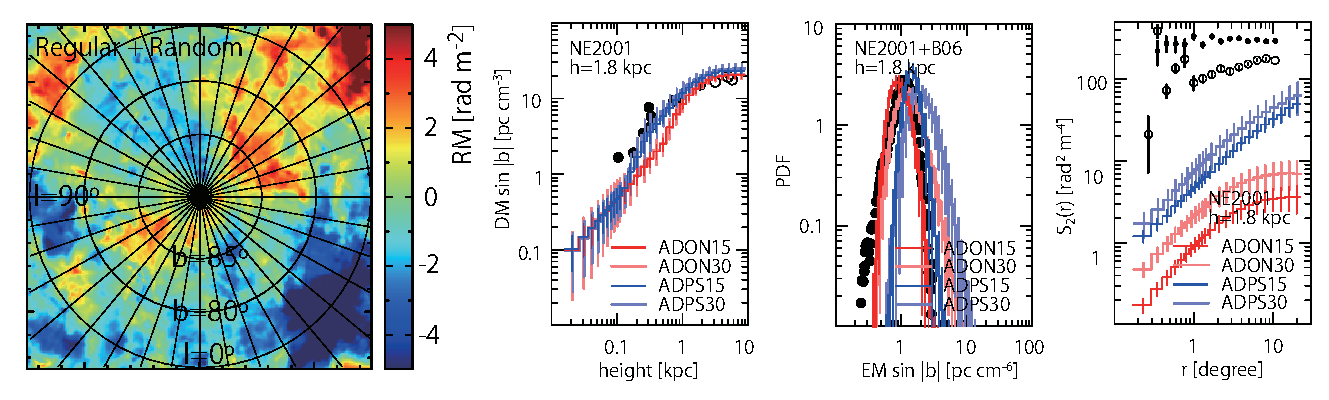
\includegraphics[width=1.0\linewidth]{ISM/c08.s3.ss6.f1.eps}
\caption{
銀極方向の天の川銀河の理論モデル。左はRMの2次元マップ。右はDM、EM、RMの観測結果(点)と理論(線)との比較。詳しくは論文を参照\citep{2013ApJ...767..150A}。
}\label{c08.s3.ss6.f1}
\end{center}
\end{figure}

\paragraph{偏波観測サイエンスとのシナジー}

一方で、上記のような偏波観測ではWIMないし宇宙線電子を探ることになり、低温の物質を探知することはできない。また当然、磁場の弱い物質は探れない。そこでこの点をH\,\textsc{i}やOHを始めとする原子・分子輝線の観測、ならびにそれらのゼーマン効果観測によって補うことは相補的といえる。例えば、日本のサイエンスとして高銀緯・ハロー方向に注目している(図\ref{c08.s3.ss6.f1})。高銀緯・ハロー方向の磁場は円盤磁場がパーカー不安定性で浮上したものが起源の可能性がある。そのプラズマの浮上は低温ガスにどのような影響を与えるのかには興味がある(一緒に浮上するのか、脇に掃き出されるのか、蒸発するのかなど)。低温ガスの構造をトレーサーとして精密に調べることで、ハロー磁場の円盤磁場浮上説を支持または制限することができれば、銀河磁場研究にとって大きな進展となる。先立って、低温物質と高温物質の住み分けあるいは共存といったことの理解と、それを考慮したセットアップでの2相の銀河円盤数値シミュレーションの実行が、最先端の課題となるだろう。


%%%%%%%%%%%%%%%%%%%%%%%%%%%%%%%%%%%%%%%%%%%%%%%
%%%%%%%%%%%%%%%%%%%%%%%%%%%%%%%%%%%%%%%%%%%%%%%
\subsection{宇宙論グループからの期待}\label{c08.s4.ss7}

\paragraph{星間物質と宇宙論}

星間物質の物理は、直接的には宇宙論の研究には無関係と思われがちであるが、今後の観測的宇宙論にとってはその理解が決定的に重要となる。高赤方偏移からのH\,\textsc{i} 21cm放射を用いた再電離期の観測では、そのシグナルより天の川銀河の星間物質からの放射の強度が4-5桁程強いであろうと見積もられている\citep{2005ApJ...625..575S}。その主な前景放射源はシンクロトロン放射であるが、熱的電子による制動放射も桁で大きく、前景放射を生み出す星間物質の正確な情報は、SKAでの再電離期の観測にとって肝であると言える\citep{2014PTEP.2014fB109I}。

\paragraph{前景放射の問題}

2014年に宇宙論業界を賑わした宇宙背景放射(CMB)のB-mode偏光観測においても、すでに天の川銀河からの前景放射が支配的な状況にある。ここでよく議論される前景偏光放射はシンクロトロン放射とダストからの熱放射である。従って、星間磁場の理解も重要となり、ここではさらに宇宙磁場グループと3グループ合わせて研究を進めることが大切だろう。また、宇宙再電離期の観測やCMBの偏光観測では銀河面から離れた柱密度の小さい方向が観測ターゲットとなるため、その前景物質の観測には大きな集光能力のあるSKAは最適である。前景放射の差し引きには、ターゲット周波数の周囲の周波数域から外挿して差し引くことが行われることが多いが、例えば視線方向に磁場、温度が異なる分子雲が複数存在した場合にはこの方法が破綻することが指摘されている\citep{2014arXiv1410.8136T}。SKAによるH\,\textsc{i}の精密な観測から各分子雲を個々に検出してモデル化することができれば、より精度の高い前景放射の差し引きが可能となり、宇宙背景放射による初期宇宙でのインフレーションの存在検証に向けてさらに一歩進むことができる。
